\documentclass[aps,prx,preprint,onecolumn,citeautoscript,footinbib]{revtex4-1}  
\synctex=1 
\bibliographystyle{apsrev4-1_custom}
\usepackage{amsmath,amssymb,bm,bbm} 
\usepackage{amsthm}
\usepackage{physics}
\usepackage{graphicx}  
\usepackage{color} 
\usepackage{comment}
\usepackage[dvipsnames]{xcolor}
\usepackage[papersize={8.5in,11in}]{geometry}
\usepackage[colorlinks=true]{hyperref}  
\usepackage[section]{placeins}
\usepackage[mathscr]{euscript}
\hypersetup{
    unicode=false,          % non-Latin characters 
    pdftoolbar=true,        % show Acrobat
    pdfmenubar=true,        % show Acrobat 
    pdffitwindow=false,     % window fit to page when opened
    pdfstartview={FitH},    % fits the width of the page to the window
    pdftitle={},    % title
    pdfauthor={},     % author
    pdfsubject={},   % subject of the document
    pdfcreator={},   % creator of the document
    pdfproducer={}, % producer of the document
    pdfkeywords={} {} {}, % list of keywords
    pdfnewwindow=true,      % links in new window
    colorlinks=true,       % false: boxed links; true: colored links
    linkcolor=magenta, %red,          % color of internal links (change box color with linkbordercolor)
    citecolor=blue,        % color of links to bibliography
    filecolor=magenta,      % color of file links
    urlcolor=blue           % color of external links
} 

\geometry{top=2.5cm, left=2cm, right=2cm, bottom=2.5cm}        

%%%%%%-- TikZ package
\usepackage{tikz}
\usepackage{tikz-cd}
\usetikzlibrary{arrows}
\usetikzlibrary{intersections}
\usetikzlibrary{shapes.geometric}
\usetikzlibrary{decorations.pathmorphing, patterns,shapes}

%---New math environment
\newtheorem{thm}{Theorem}[section]
\newtheorem{lemma}{Lemma}[section]
\newtheorem{prop}[thm]{Proposition}
\newtheorem{cor}[thm]{Corollary}

\newenvironment{pf}[1][Proof]{\begin{trivlist}
\item[\hskip \labelsep {\bfseries #1}]}{\end{trivlist}}
\newenvironment{defn}[1][Definition]{\begin{trivlist}
\item[\hskip \labelsep {\bfseries #1}]}{\end{trivlist}}
\newenvironment{ex}[1][Example]{\begin{trivlist}
\item[\hskip \labelsep {\bfseries #1}]}{\end{trivlist}}
\newenvironment{rmk}[1][Remark]{\begin{trivlist}
\item[\hskip \labelsep {\bfseries #1}]}{\end{trivlist}}

\renewcommand{\bar}{\overline}
\renewcommand{\tilde}{\widetilde}
\renewcommand{\hat}{\widehat}
\renewcommand{\leq}{\leqslant}
\renewcommand{\geq}{\geqslant}
\renewcommand{\Re}{\operatorname{Re}}
\renewcommand{\Im}{\operatorname{Im}}

\newcommand{\Sch}{\operatorname{Sch}}
\newcommand{\Li}{\operatorname{Li}}

\newcommand{\nn}{\nonumber}
\newcommand{\Pf}{\operatorname{Pf}}
\newcommand{\const}{\operatorname{const}}
\newcommand{\OTOC}{\text{OTOC}}

\newcommand{\calD}{\mathcal{D}}
\newcommand{\UU}{\operatorname{U}}
\newcommand{\SU}{\operatorname{SU}}
\newcommand{\SO}{\operatorname{SO}}
\newcommand{\SL}{\operatorname{SL}}
\newcommand{\GL}{\operatorname{GL}}
\newcommand{\PSL}{\operatorname{PSL}}
%---- marcos for math font 
\newcommand{\CC}{\mathbb{C}}
\newcommand{\RR}{\mathbb{R}}
\newcommand{\HH}{\mathbb{H}}
\newcommand{\ZZ}{\mathbb{Z}}

\newcommand{\calE}{\mathscr{E}}%upright Euler script 

\newcommand{\YG}[1]{\textcolor{blue}{#1}}
\def\arraystretch{1.5}
\newcommand{\eff}{{\rm eff}}

\linespread{1.3}
\usepackage{amsfonts}
\usepackage{upgreek}
\usepackage{slashed}
\usepackage{latexsym}
%\usepackage{showkeys}
\usepackage{todonotes}

\newcommand{\beq}{\begin{equation}}
\newcommand{\eeq}{\end{equation}}
\def\bea{\begin{eqnarray}}
\def\eea{\end{eqnarray}}
\newcommand{\sgn}{\operatorname{sgn}}
\newcommand{\note}[1]{{\color{red}[#1]}}

\begin{document}
\section{Overall Idea}
In calculating the four-point function of the SYK model, we find an enhanced contribution which can be interpreted as arising from reparameterizations of the Green's function with a cost given by the Schwarzian action. This Schwarzian contribution should manifest itself in general $2n$-point functions, with a $2n$-point function containing information about the $n$-point vertex of the Schwarzian theory. As we want to show, the way these vertices arise is not obvious. The expansion parameter of the Schwarzian action is $\beta J/N$, with propagators giving a factor of $\beta J/N$ and vertices giving $N/\beta J$. If we calculate the $2n$-point functions using ladder diagrams, the factor of $N$ in the vertex simply arises from summing over indices. However, the $1/\beta J$ suppression in the vertex is not at all obvious. Understanding how this arises might be useful because it shows which diagrams give soft mode contributions, and may also be helpful in calculating higher order corrections, i.e. $1/N^2$ corrections to the four-point function.
\section{Contact Diagrams}
\subsection{Contributions from the $h=2$ subspace}
Here, we study the $h=2$ contribution to the contact diagrams of the six-point function, shown in Fig.~\ref{fig:contact}. We do not except the Schwarzian action to contribute to these diagrams, since the Schwarzian should contribute to arbitrary $2n$-point functions for any $q$, with the only $q$-dependence being some simple coefficients. In contrast, these contact diagrams only support a maximum of $q$ outgoing ladders, so they qualitatively behave differently from what we'd expect.
\begin{figure}
    \centering
    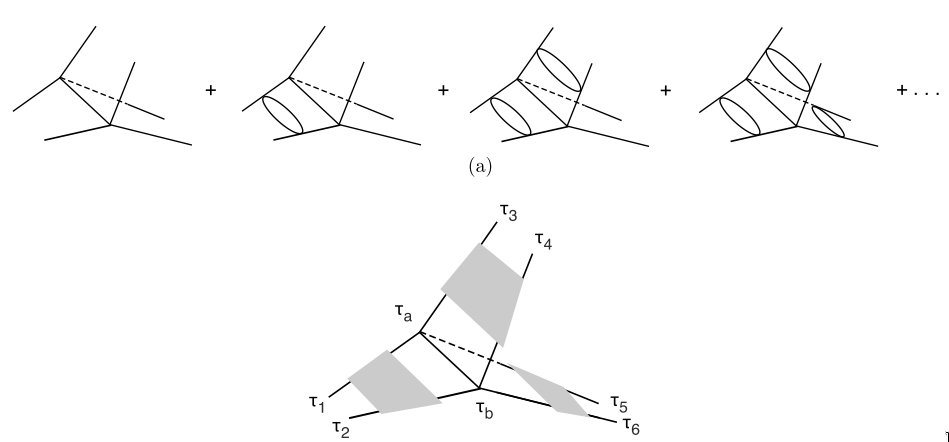
\includegraphics[width=0.7\textwidth]{contact.png}
    \caption{Contact diagrams (figure taken from Gross/Rosenhaus)}
    \label{fig:contact}
\end{figure}
The contribution of these diagrams can be obtained by connecting together three ladders at a ``contact" vertex, and integrating over the intermediate times. 
\begin{equation}
    \begin{aligned}
        \mathcal{S} = \int \dd{\tau_a} \dd{\tau_b} G^{q-3}(\tau_ab) \mathcal{F}(\tau_1, \tau_2, \tau_a, \tau_b)\mathcal{F}(\tau_3, \tau_4, \tau_a, \tau_b)\mathcal{F}(\tau_5, \tau_6, \tau_a, \tau_b)
    \end{aligned}
\end{equation}
We are interested in the $h=2$ contribution to this class of diagrams, given by
\begin{equation}
 \left[(q-1) J^2 G^{\frac{q-2}{2}}(\tau_{12})  G^{\frac{q-2}{2}}(\tau_{34})\right] \mathcal{F}(\tau_1, \tau_2, \tau_3, \tau_4) = 2 \sum_n \frac{k(2, n)}{1-k(2, n)} \Psi_{2, n}(\tau_1, \tau_2) \Psi_{2, n}^*(\tau_3, \tau_4)\,.
 \label{eq:softModeFourPoint}
\end{equation}
Isolating the $\tau_{a,b}$ dependence of the integrand, we have a sum over $n_1, n_2, n_3$ integrals of the form
\begin{equation}
    \begin{aligned}
         \int \dd{\tau_a} \dd{\tau_b} G^{-q/2} \Psi_{2, n_1}(\tau_a, \tau_b) \Psi_{2, n_2}(\tau_a, \tau_b) \Psi_{2, n_3}(\tau_a, \tau_b)\,.
         \label{eq:contactIntegral}
    \end{aligned}
\end{equation}
Using the conformal expressions for $\Psi_{2, n_i}$, one can check in Mathematica that this integral vanishes for all $n_i$. I have not had the chance to derive this analytically - it's not immediately obvious why this has to be true, but it probably follows straightforwardly from some trigonometric identities. 

We've shown that these diagrams vanish at leading order, but we expect this to be true regardless of whether contact diagrams contribute to the Schwarzian action, since these contributions are proportional to $(\beta J)^3/N^2$. What we still need to show is that the first-order corrections, which are proportional to $(\beta J/N)^2$, also vanish. These come from considering the $\frac{1}{\beta J}$ corrections to both the kernel eigenfunctions and the Green's function in Eq.~\ref{eq:contactIntegral}.  \note{These calculations are copied from a note I wrote a few months ago. I had some difficulty understanding these notes when I read them recently, so I'm not confident that my derivation here is completely accurate, but I think the overall idea is right - the coefficients just might be off.}  We first calculate the corrections to the $h=2$ kernel eigenfunctions. In the $q \rightarrow \infty$ limit, the kernel eigenfunctions are known exactly:
\begin{equation}
    \begin{aligned}
        \Psi_{h, n}(\tau_1, \tau_2) &= \frac{e^{iny}}{\sin\frac{\tilde{x}}{2}} \psi_{h, n}(x) \quad y = \frac{\tau_1 + \tau_2}{2} \quad x = \tau_1 = \tau_2 \quad \tilde{x} = v x + (1-v)\pi
  \\
  \psi_{h,n}(x) &\sim \left( \sin\frac{\tilde{x}}{2} \right)^h F\left( \frac{h-\tilde{n}}{2}, \frac{h + \tilde{n}}{2}, \frac{1}{2}, \cos^2\frac{\tilde{x}}{2} \right) \quad \tilde{n} = \frac{n}{v} \quad (n \text{ even })
  \\
  \psi_{h,n}(x) &\sim \cos \frac{\tilde{x}}{2} \left( \sin\frac{\tilde{x}}{2} \right)^h F\left( \frac{1+h-\tilde{n}}{2}, \frac{1+h + \tilde{n}}{2}, \frac{3}{2}, \cos^2\frac{\tilde{x}}{2} \right) \quad \tilde{n} = \frac{n}{v} \quad (n \text{ odd })\end{aligned}
\end{equation}
The $h=2$ contribution is shifted to $h=2 + \abs{n} \frac{1-v}{v}$ in order for there to be no divergence as $x \rightarrow 0$.
From these exact solutions, we have
\begin{equation}
    \delta \Psi_{2, n} = \frac{1}{\beta J} \partial_{1/\beta J} \Psi^{exact}_{2,n}\Big|_{\beta J = \infty} = \frac{1}{\beta J} \pdv{v}{1/\beta J} \pdv{v} \Psi^{exact}_{2,n}\Big|_{v=1}\,.
\end{equation}
This lets us recast the three different contributions as
\begin{equation}
    \frac{1}{\beta J} \pdv{v}{(\beta J)^{-1}} \pdv{v}\left( \int \dd{\tau_a} \dd{\tau_b}   \Psi_{2, n_1} \Psi_{2, n_2}\Psi_{2, n_3} G_c^{-q/2}\right) \Big|_{v=1}
\end{equation}
Doing the integral over $\tau_a + \tau_b$, this gives
\begin{equation}
    \frac{2\pi}{\beta J} \pdv{v}{(\beta J)^{-1}} \pdv{v}\left( \int \dd{x}  \psi_{2, n_1} \psi_{2, n_2} \psi_{2, n_3} G_c^{-q/2}\right) \Big|_{v=1}
\end{equation}
where we have absorbed the factors of $\left(\sin\frac{\tilde{x}}{2}\right)^{-1}$ into the definition of $\psi$. We find numerically that this integral vanishes if we substitute $\tilde{x} \rightarrow x$ in the equations for $\psi$. This is likely due to the same reason that the conformal vertex vanishes, although the two integrals are not exactly the same since we still have the rescaling $n \rightarrow n/v$. 
Anyways, this means that if we take $\epsilon = 1-v$ and expand in powers of $\epsilon$, we can obtain the following relation
\begin{equation*}
  \begin{aligned}
    &\int_0^{2\pi} \dd{x}  \psi_{2, n_1}(x) \psi_{2, n_2}(x) \psi_{2, n_3}(x) G_c^{-q/2}(x) 
    \\
    &= \frac{\epsilon}{b^{q/2}} \int_{-\epsilon/2}^{2\pi + \pi \epsilon} (x-\pi) \psi_{2, n_1}(x \equiv \tilde{x}) \psi_{2, n_2}(x \equiv \tilde{x})\psi_{2, n_3}(x \equiv \tilde{x})  \cos\left( \frac{x}{2} \right) 
  \\
  &- \left( \int_{-\epsilon/2}^0 + \int_{2\pi}^{2\pi + \epsilon \pi} \right) \dd{x}\psi^c_{2, n_1}(x) \psi_{2, n_2}^c(x)\psi_{2, n_3}^{c}(x)  G_c^{-q/2}(x) + \order{\epsilon^2}
\end{aligned}
\end{equation*}
We are interested in evaluation the derivative of this expression, which is
\begin{equation*}
  \begin{aligned}
    &\pdv{v} \left[\int_0^{2\pi} \dd{x} \psi^c_{2, n_1}(x) \psi_{2, n_2}^c(x)\psi_{2, n_3}^{c}(x)  G_c^{-q/2}(x)\right]\Big|_{v=1} 
    \\
    &= -\lim_{\epsilon \rightarrow 0} \frac{1}{\epsilon}\int_0^{2\pi} \dd{x} \psi^c_{2, n_1}(x) \psi_{2, n_2}^c(x)\psi_{2, n_3}^{c}(x)  G_c^{-q/2}(x) 
    \\
    &= - \frac{1}{b^{q/2}} \int_{0}^{2\pi} (x-\pi) \psi^c_{2, n_1}(x) \psi_{2, n_2}^c(x)\psi_{2, n_3}^{c}(x)  \cos\left( \frac{x}{2} \right)\,.
  \end{aligned}
\end{equation*}
The ``boundary'' terms from this derivative vanish because $\psi^c_{2, n}(0) = 0$. For general $q$, the correction is still the same, but with an additional prefactor of $\frac{\alpha_G q}{2}$. This exactly cancels the correction coming from the Green's function
\begin{equation}
    G^{-q/2} = G_c^{-q/2} \left(1 + \frac{\delta G}{G_c}\right)^{-q/2} \approx G_c^{-q/2} + G_c^{-q/2}\frac{\alpha_G q}{2\beta J} \left[2 + \frac{\pi - \abs{\tau}}{\tan{\frac{\abs{\tau}}{2}}}\right] 
\end{equation}
\subsection{Contributions from the $h \neq 2$ subspace}
If all three ladders have a soft mode, the $(\beta J/N)^2$ contributions from the contact diagrams vanish. If we replace one of the one of the soft modes with an $h \neq 2$ mode, we obtain a diagram that naively contributes at order $(\beta J/N)^2$, assuming the leading-order vertex does not vanish. The vertices in these cases would take the form
\begin{equation}
    V_{h, n_1, n_2, n_3} \sim \int \dd{\tau_a} \dd{\tau_b} G^{-q/2}(\tau_{ab}) \Psi_{h, n_1}(\tau_a, \tau_b) \Psi_{2, n_2}(\tau_a, \tau_b) \Psi_{2, n_3}(\tau_a, \tau_b)\,.
    \label{eq:contactVertexhneq2}
\end{equation}
Calculating these vertices in Mathematica shows that, at least for the discrete series, these vertices generically have some non-zero value when the conformal solutions are used (in fact, Mathematica is able to do the integrals exactly, and at least for the discrete series it should be possible to obtain an analytic expression as a function of $h$ and $n_i$). I have not looked into this extensively yet, but it seems like there are three possibilities:
\begin{itemize}
    \item These sorts of diagrams also correspond to the Schwarzian action and must be included in order to get the answer for the six-point function that we would expect from a pure Schwarzian calculation (unlikely).
    \item These diagrams ultimately vanish in some non-trivial manner when the summation/integration over $h$ is carried out (possible, but would be very non-trivial - although one possibility is that for a fixed $h$ and $n_i$, these diagrams are directly cancelled by the planar diagrams with the same $h$, $n_i$).
    \item There are additional $(\beta J/N)^2$ contributions to the six-point function that do not come purely from the Schwarzian sector. Roughly speaking, they correspond to an $\order{1}$ vertex coupling between the soft mode and the other modes. It's not clear to me yet whether this is an obvious contradiction or a possibility, but it seems like an interesting result if it is possible.
\end{itemize}
It might also be possible to understand integrals like Eq.~\ref{eq:contactVertexhneq2} on the basis of $\SL(2, \mathbb{R})$ representations, by understanding the tensor decomposition of two of the eigenfunctions and using the orthogonality of different representations. This is difficult though, as the kernel eigenfunctions $\Psi_h$ are scalar eigenfunctions, or $\nu$-spinors with $\nu=0$, on the hyperbolic plane $\text{H}_2$. In the irreducible representation $\mathcal{D}^\pm_h$, the range of $\nu$ is restricted to $\abs{\nu} > h$. This means that, even though one can obtain equations for $\Psi_h$ through $\SL(2, \mathbb{R})$ representations by computing the eigenfunctions of $\nu$-spinors on $\text{H}_2$ and setting $\nu=0$, the resulting functions don't actually correspond to matrix elements of unitary representations in any formal group-theoretic sense, and therefore the normal approach of tensor decompositions does not work.
\section{Planar Diagrams}
\subsection{Amputated Ladder Approach}
The planar contributions, shown in Fig.~\ref{fig:planar} to the six-point function can be expressed as
\begin{equation}
    \mathcal{S} = \int \dd{\tau_a} \dd{\tau_b} \dd{\tau_c} \mathcal{F}_{\text{amp}}(\tau_1, \tau_2, \tau_a, \tau_b)
     \mathcal{F}_{\text{amp}}(\tau_4, \tau_3, \tau_c, \tau_a)
      \mathcal{F}_{\text{amp}}(\tau_5, \tau_6, \tau_b, \tau_c)\,,
      \label{eq:planarIntegral}
\end{equation}
\begin{figure}
    \centering
    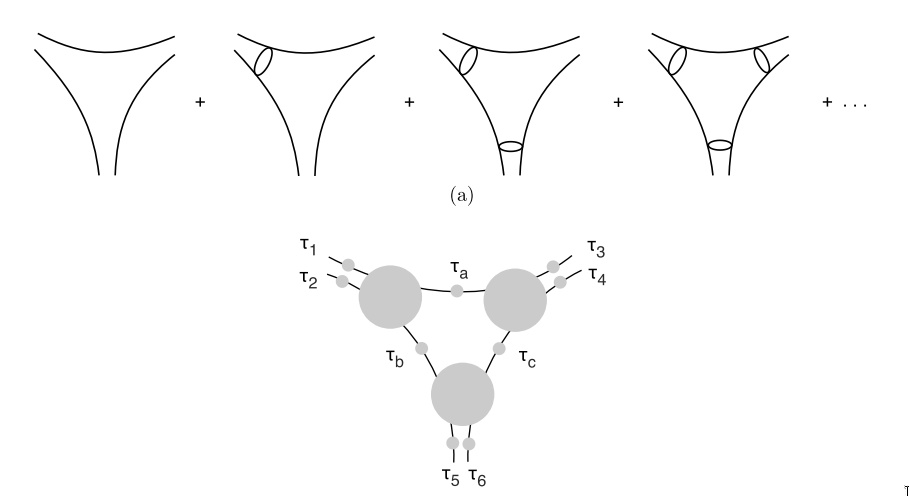
\includegraphics[width=0.7\textwidth]{planar.png}
    \caption{Planar diagrams (figure taken from Gross/Rosenhaus)}
    \label{fig:planar}
\end{figure}
where $\mathcal{F}_{\text{amp}}$ is an ``amputated" ladder diagram, essentially a ladder diagram with one of the end propagators removed,
\begin{equation}
    \mathcal{F}_{\text{amp}}(\tau_1, \tau_2, \tau_3, \tau_4) = - \int \dd{\tau_0} \mathcal{F}(\tau_1, \tau_2, \tau_3, \tau_0) \Sigma(\tau_{04})\,.
\end{equation}
In the conformal limit, we can replace $\Sigma(\tau_{40})$ with $J^2 G(\tau_{40})^{q-1}$.

We are interested in the $h=2$ contribution to this class of diagrams, given by
\begin{equation}
 \left[(q-1) J^2 G^{\frac{q-2}{2}}(\tau_{12})  G^{\frac{q-2}{2}}(\tau_{34})\right] \mathcal{F}(\tau_1, \tau_2, \tau_3, \tau_4) = 2 \sum_n \frac{k(2, n)}{1-k(2, n)} \Psi_{2, n}(\tau_1, \tau_2) \Psi_{2, n}^*(\tau_3, \tau_4)\,.
 \label{eq:softModeFourPoint}
\end{equation}
Substituting this equation into Eq.~\ref{eq:planarIntegral}, we find that $S$ is proportional to the integrals
\begin{equation}
\begin{aligned}
    \mathcal{S} &\sim \sum_{n_1, n_2, n_3} \left[\prod_{i=1,2,3}\frac{k(2, n_i)}{1-k(2, n_i)}\right]\Psi_{2, n_1}(\tau_1, \tau_2) \Psi_{2, n_2}(\tau_3, \tau_4) \Psi_{2, n_3}(\tau_5, \tau_6)
    \\
    &\times \int \Psi_{2, n_1}(\tau_a, \tau_b) \Sigma(\tau_b, \tau_c) \Psi_{2, n_2}(\tau_c, \tau_d) \Sigma(\tau_d, \tau_e) \Psi_{2, n_3}(\tau_e, \tau_f)\Sigma(\tau_f, \tau_a)
    \end{aligned}
\end{equation}
where the integral is taken over all times in the integrand. We omit the additional factors of $G^{\frac{q-2}{2}}$ coming from Eq.~\ref{eq:softModeFourPoint} for now, as they'll eventually be cancelled out by some other factors. 

Roughly speaking, if we think of the incoming ladders as propagators with coefficients $\frac{k(2, n_i)}{1-k(2, n_i)} \sim \beta J$, the vertex is
\begin{equation}
    V_{n_1, n_2, n_3} \sim \int \Psi_{2, n_1}(\tau_a, \tau_b) \Sigma(\tau_b, \tau_c) \Psi_{2, n_2}(\tau_c, \tau_d) \Sigma(\tau_d, \tau_e) \Psi_{2, n_3}(\tau_e, \tau_f)\Sigma(\tau_f, \tau_a)\,.
    \label{eq:vertex}
\end{equation}
We assume that in order for the calculations to match up with the Schwarzian calculations, the conformal result for $V_{n_1, n_2, n_3}$ must vanish, with subleading $\sim 1/\beta J$ contributions giving the intended vertex. Strictly speaking, this doesn't have to be true. It could be possible that the conformal result for $V$ is non-zero, but only the total contribution after summing over all momentum $n_i$ is zero. I very much hope this isn't the case...but I'm not sure if we can rule out the possibility. Unlike the contact diagrams, where everything was finite, the vertex for the planar diagrams as given in Eq.~\ref{eq:vertex} is poorly behaved due to the divergences in $\Sigma$ as the two times become coincident, so one cannot simply check numerically whether the leading order result for $V$ is zero.

The vertex $V_{n_1, n_2, n_3}$ is only non-zero when $n_1 + n_2 + n_3 = 0$, although this fact is not obvious from Eq.~\ref{eq:vertex}. This derivation is given in the appendix - it involves doing the integrals of $V$ in a way which I don't think is helpful for actually computing the final solution, but does allow us to extract a factor of $\delta_{n_1 + n_2 + n_3, 0}$.

A fact that seems relevant to the vanishing of $V$ at leading order is the fact that the conformal $h=2$ eigenfunctions can be expressed as linear reparameterizations of the Green's function. Explicitly,
\begin{equation}
    \Psi_{2, n} \sim \abs{G^{\frac{q-2}{2}}} \delta_{\epsilon} G 
\end{equation}
where $\delta_\epsilon G$ is the change in $G$ from an infinitesimal reparameterization, $\tau \rightarrow \tau + \epsilon(\tau)$, with $\epsilon(\tau) \sim e^{in\tau}$. This additional factor of $G^{\frac{q-2}{2}}$ cancels out the negelected factors of $G$ from Eq.~\ref{eq:softModeFourPoint} that we were ignoring, leading to 
\begin{equation}
\begin{aligned}
    V_{n_1, n_2, n_3} &\sim \int \delta_1 G(\tau_a, \tau_b) \Sigma(\tau_b, \tau_c) \delta_2 G(\tau_c, \tau_d) \Sigma(\tau_d, \tau_e) \delta_3 G(\tau_e, \tau_f)\Sigma(\tau_f, \tau_a) + \order{1/\beta J}
    \\
    &= \Tr \left[ (\delta_1 G) \Sigma (\delta_2 G) \Sigma (\delta_3 G) \Sigma \right] + \order{1/\beta J}\,.
    \label{eq:vertexSimplified}
    \end{aligned}
\end{equation}
In the last expression, we write the integrals as a trace, with matrix multiplication representing convolution. We write $\delta_i G \equiv \delta_\epsilon G$, where $\epsilon(\tau) \sim e^{i n_i \tau}$. This expression is also easily generalized to the $2n$-point function vertex, with the trace containing $n$ copies of Green's functions and self-energies.

Another useful fact is that the reparameterization-invariance of the conformal Schwinger-Dyson equations implies
\begin{equation}
    0 = (\delta_\epsilon G) \Sigma + G (\delta_\epsilon \Sigma)
    \label{eq:sdInvarianceCondition}
\end{equation}
where again, the convolution in these equations is implicit. This comes from the fact that $(G_c + \delta_\epsilon G_c)$ and $(\Sigma_c + \delta_\epsilon \Sigma_c)$ must also satisfy the Schwinger-Dyson equations. This means that we can essentially move around the reparameterizations in Eq.~\ref{eq:vertexSimplified} at the cost of a minus sign.
With this, we can simplify the expression using the Schwinger-Dyson equations,
\begin{equation}
    V_{n_1, n_2, n_3} \sim \Tr\left[(\delta_1 G) (\delta_2 \Sigma) (\delta_3 G) \Sigma\right]
\end{equation}
My understanding is that one can also derive conditions similar to Eq.~\ref{eq:sdInvarianceCondition} under multiple reparameterizations, but I'm not sure if I'm missing some subtlety. If $(G_c + \delta_1 G_c)$ satisfies the Schwinger-Dyson equations, then requiring that $G_c + \delta_1 G_c + \delta_2(G_c + \delta_1 G_c)$ also satisfies the Schwinger-Dyson equations leads to the equality
\begin{equation}
    \delta_1 G \delta_2 \Sigma + \delta_2 G \delta_1 \Sigma + (\delta_1 \delta_2 G) \Sigma + G (\delta_1 \delta_2 \Sigma) = 0
\end{equation}
from which we can obtain
\begin{equation}
\begin{aligned}
    \Tr \left[ (\delta_1 G) (\delta_2 \Sigma) (\delta_3 G) \Sigma \right] &= - \Tr[(\delta_2 G)(\delta_1 \Sigma)(\delta_3 G) \Sigma] - \Tr[(\delta_1 \delta_2 G) \Sigma (\delta_3 G) \Sigma] - \Tr[G (\delta_1 \delta_2 \Sigma) (\delta_3 G)\Sigma ]
    \\
     &= -\Tr[(\delta_2 G)(\delta_1 \Sigma)(\delta_3 G) \Sigma] + \Tr[(\delta_1 \delta_2 G) (\delta_3 \Sigma) G \Sigma] - \Tr[G (\delta_1 \delta_2 \Sigma) (\delta_3 G)\Sigma]
    \\
    &= -\Tr[(\delta_2 G)(\delta_1 \Sigma)(\delta_3 G) \Sigma] - \Tr[(\delta_1 \delta_2 G) (\delta_3 \Sigma)] - \Tr[(\delta_1 \delta_2 \Sigma) (\delta_3 G)]
    \end{aligned}
\end{equation}
where in the last line we use the fact that $G \Sigma = -1$ \note{On the last line, the final term on the RHS should have a plus sign instead of a minus sign, which messes up the rest of the derivation...}.
By permutation invariance of the three momentum, we can assume the first two terms on each side of the equality are the same, giving
\begin{equation}
    V_{n_1, n_2, n_3} \sim \Tr[(\delta_1 \delta_2 G) (\delta_3 \Sigma)] + \Tr[(\delta_1 \delta_2 \Sigma) (\delta_3 G)]\,.
    \label{eq:planarReduced}
\end{equation}
Now, we use the identity that comes from requiring that the Schwinger-Dyson equations are invariant under three reparameterizations. This gives
\begin{equation}
   (\delta_1 \delta_2 G)(\delta_3 \Sigma) + (\delta_3 G)(\delta_1 \delta_2 \Sigma) + \text{additional permutations} + (\delta_1 \delta_2 \delta_3 G)\Sigma + G (\delta_1 \delta_2 \delta_3 \Sigma) = 0
   \label{eq:reparamIdentiy}
\end{equation}
We also have that $\delta_1 \delta_2 \delta_3 G = \delta_1 \delta_2 \delta_3 \Sigma = 0$, which is a consequence of $n_1 + n_2 + n_3 = 0$. By permutation invariance momentum, this finally gives $V_{n_1, n_2, n_3} = 0 + \order{1/\beta J}$. 

\subsection{Kernel Approach}
An alternate derivation of the planar diagrams can be used, which closely mirrors the four-point function derivation. We start with the $1/N^2$ contribution to the six-point function with no rungs, $\mathcal{F}_0$, shown in Fig.~\ref{fig:f0}. The planar diagrams are generated by acting on the three "edges" of $\mathcal{F}_0$ with kernel operators. This leads to
\begin{equation}
    \begin{aligned}
        \mathcal{F}^{\mu \nu \sigma} = \sum_{n, m, l=0} K_{\mu \delta}^n K_{\nu \epsilon}^m K_{\sigma \lambda}^l \mathcal{F}_0^{\delta \epsilon \lambda} = \frac{1}{1-K}\frac{1}{1-K}\frac{1}{1-K} \mathcal{F}_0
    \end{aligned}
\end{equation}
Where each index corresponds to two times. In the final expression, each factor of $\frac{1}{1-K}$ acts on two different times. 
\begin{figure}
    \centering
    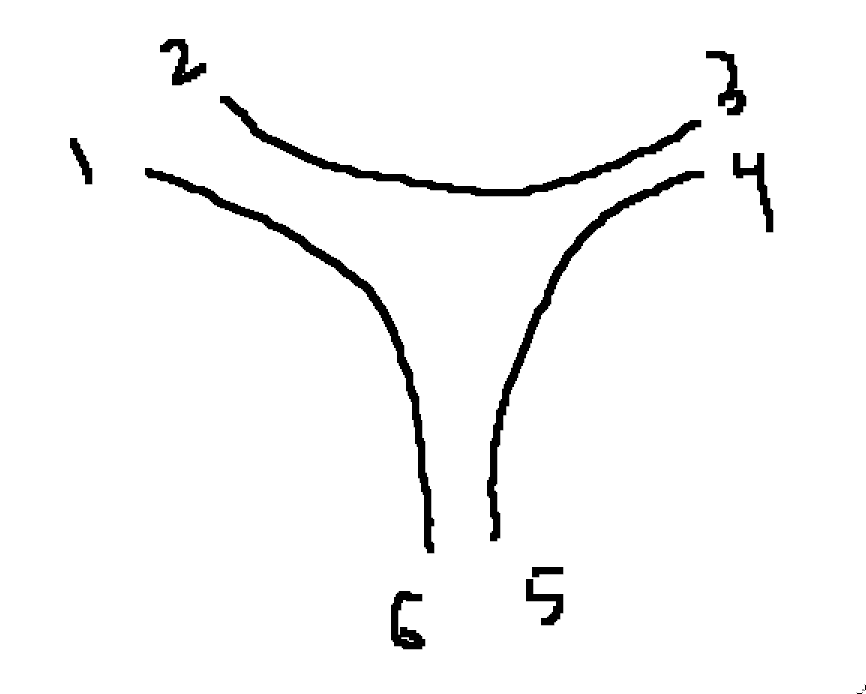
\includegraphics[width=0.5\textwidth]{f0}
    \caption{The diagram corresponding to $\mathcal{F}_0$. If this kernel approach proves to be useful, I'll make an actual figure for this.}
    \label{fig:f0}
\end{figure}
Similar to the four-point approach, we can solve this by finding the eigenfunctions of $\frac{1}{1-K}\frac{1}{1-K}\frac{1}{1-K}$, denoted as $\Psi_i$ with eigenvalue $\lambda_i$ which are just tensor products of ladder eigenfunctions. We then have
\begin{equation}
    \begin{aligned}
        \mathcal{F} = \sum_i \frac{\lambda_i \Psi_i \langle \mathcal{F}_0, \Psi_i\rangle}{\langle \Psi_i, \Psi_i\rangle}
    \end{aligned}
\end{equation}
The soft mode contribution to this is given by $\Psi_i = \Psi_{2, n_1} \otimes \Psi_{2, n_2} \otimes \Psi_{2, n_3}$, where we have reverted back to using eigenfunctions of the normal kernel. Each factor of $\frac{1}{1-k(2, n)}$ corresponds to a propagator (recall that to leading order, $\frac{K}{1-K} = \frac{1}{1-K}$ for the $h=2$ contributions), from which we conclude that the vertex is simply
\begin{equation}
    \begin{aligned}
    V_{n_1, n_2, n_3} &= \langle \mathcal{F}_0,  \Psi_{2, n_1} \otimes \Psi_{2, n_2} \otimes \Psi_{2, n_3} \rangle
    \\
    &= \int G(\tau_a, \tau_b) \delta_1 G(\tau_b, \tau_c) G(\tau_c, \tau_d) \delta_2 G(\tau_d, \tau_e) G(\tau_e, \tau_f) \delta_3 G(\tau_f, \tau_a) 
    \\
    &= \Tr\left[G (\delta_1 G) G (\delta_2 G) G (\delta_3 G)G \right]
    \end{aligned}
\end{equation}
which is essentially the same form of the integral we obtained earlier, but with $\Sigma$'s replaced by $G$'s. These two integrals are not exactly equal, since there are overall coefficients that we're neglecting - I think the two integrals only differ by a factor of $\left[(q-1)J^2\right]^3$, but there are likely some small additional coefficients that I'm missing.
\appendix
\section{Explicit form of linearized reparameterizations}
It might be necessary to use the explicit form of the reparameterzations,
\begin{equation}
\begin{aligned}
    \delta_i G(\tau_1, \tau_2) &= \abs{G(\tau_{12})} e^{-in_i \frac{\tau_1 + \tau_2}{2}} f_n(\tau_{12})\,,
    \\
    \delta_i \Sigma(\tau_1, \tau_2) &\sim  \abs{\Sigma(\tau_{12})} e^{-in_i \frac{\tau_1 + \tau_2}{2}} f_n(\tau_{12})\,,
    \\
    f_n(x) &= \frac{\sin\frac{nx}{2}}{\tan \frac{x}{2}} - n \cos \frac{nx}{2}\,.
    \end{aligned}
\end{equation}
A useful fact about $f_n$ is that when $n$ is even, its Fourier coefficients take on a simple form, $c_m = 1$ when $\abs{c_m} < \frac{n}{2}$, $c_m = -\frac{n-1}{2}$ when $\abs{c_m} = \frac{n}{2}$, and $c_m = 0$ otherwise. A similar statement is true for odd $n$, except with the Fourier series done with half-integer (fermionic) frequencies.

\section{Momentum Conservation}
The vertex $V_{n_1, n_2, n_3}$ is only non-zero when  $n_1 + n_2 + n_3 = 0$. Defining 
\begin{equation*}
    \begin{aligned}
    t_1 &= \tau_a - \tau_b
    \\
    T_1 &= \frac{\tau_a + \tau_b}{2}
    \\
    t_2 &= \tau_c - \tau_d
    \\
    T_2 &= \frac{\tau_c + \tau_d}{2}
    \\
    t_3 &= \tau_e - \tau_f
    \\
    T_3 &= \frac{\tau_e + \tau_f}{2}
    \\
    \end{aligned}
\end{equation*}
we can rewrite the vertex as
\begin{equation*}
    \begin{aligned}
    V_{n_1, n_2, n_3} &= \int \exp\left[-i(n_1 T_1 + n_2 T_2 + n_3 T_3)\right] \psi_{n_1}(t_1) \Sigma\left(T_1 - \frac{t_1+t_2}{2} - T_2\right)
    \\
    &\times\psi_{n_2}(t_2)\Sigma\left(T_2 - \frac{t_2+t_3}{2} - T_3\right)\psi_{n_3}(t_3) \Sigma\left(T_3 - \frac{t_3+t_1}{2} - T_1\right)\,.
    \end{aligned}
\end{equation*}
Now the integrals over $T_i$ can be done, essentially consituting Fourier transforms. We first carry out the integral over $T_1$, which two of the self-energies are dependent on. This Fourier transform is subtle, since the product of the two self-energies is periodic, but the individual self-energies are anti-periodic. One can show a modified version of the convolution property still holds. Let $f(t)$ and $g(t)$ be two anti-periodic functions with Fourier transforms $f(\omega_n)$ and $g(\omega_n)$, with $\omega_n = n + \frac{1}{2}$. Then,
\begin{equation*}
\begin{aligned}
    \int_0^{2\pi} \dd{t} e^{-i n t} f(t) g(t) = \sum_{m_1, m_2} \int_0^{2\pi} \dd{t} e^{-i (n - m_1 - m_2 - 1)t} f(\omega_{m_1})g(\omega_{m_2}) = \sum_m f(\omega_{m})g(\omega_{n-m-1})\,.
    \end{aligned}
\end{equation*}
We also have the usual property of translation - if $f(t)$ is anti-periodic with Fourier coefficients $f(\omega_n)$, then $f(t-a)$ has coefficients $e^{-i\left(n+\frac{1}{2}\right)a}f(\omega_n)$ 
So,
\begin{equation*}
    \begin{aligned}
        V_{n_1, n_2, n_3} &=-\sum_m  \int \exp\left[-i \left(n_2 T_2 + n_3 T_3 + \left(m + \frac{1}{2}\right)\left(\frac{t_1 + t_2}{2} + T_2\right) +  \left(n_1-m - \frac{1}{2}\right)\left(\frac{t_1 + t_3}{2} + T_3\right)\right)\right]
        \\
        &\times \frac{\Sigma\left(T_2 - \frac{t_2 + t_3}{2} - T_3\right)}{G(\omega_m) G(\omega_{m-n_1})}\psi_{n_1}(t_1)\psi_{n_2}(t_2)\psi_{n_3}(t_3)
        \\
        &= \sum_m \int %\exp\left[-i(n_3 T_3 + \left(m + \frac{1}{2}\right)\left(\frac{t_1 + t_2}{2}\right) +  \left(n_1-m - \frac{1}{2}\right)\left(\frac{t_1 + t_3}{2} + T_3\right) + \left(n_2 + m + \frac{1}{2}\right) \left(\frac{t_2 + t_3}{2} + T_3\right)\right]
        \exp\left[-i\left(T_3(n_1 + n_2 + n_3) + t_1 \frac{n_1}{2} + t_2 \left(\frac{n_2}{2}+m+1\right) + t_3\left(\frac{n_1 + n_2}{2}\right)\right)\right]
        \\
        &\times \frac{\psi_{n_1}(t_1) \psi_{n_2}(t_2) \psi_{n_3}(t_3)}{G(\omega_m) G(\omega_{m-{n_1}})G(\omega_{m + n_2})}
        \\
        &= \delta_{n_1 + n_2 + n_3} \sum_m\int  \exp\left[-i\left(t_1 \frac{n_1}{2} + t_2 \left(\frac{n_2}{2}+m+1\right) - t_3\left(\frac{n_3}{2}\right)\right)\right]\frac{\psi_{n_1}(t_1) \psi_{n_2}(t_2) \psi_{n_3}(t_3)}{G(\omega_m) G(\omega_{m-{n_1}})G(\omega_{m + n_2})}
    \end{aligned}
\end{equation*}
It's not obvious how to complete this calculation. The remaining integrals are Fourier transforms with integer (half-integer) frequencies when $n_i$ is even (odd). We know that $\psi_{n_i} \sim G \times f_{n_i}$, where $G$ is anti-periodic and $f_{n_i}$ has a simple Fourier series if we take it to be periodic (anti-periodic) when $n_i$ is even (odd). But the anti-periodicity of $G$ spoils this simplification, since even (odd) $n_i$ forces us to take the the Fourier transform of $f_i$ with respect to half-integer (integer) frequencies.
\end{document}
